\documentclass[conference]{IEEEtran}
\IEEEoverridecommandlockouts

\usepackage{cite}
\usepackage{amsmath,amssymb,amsfonts}
\usepackage{algorithmic}
\usepackage{graphicx}
\usepackage{textcomp}
\usepackage{xcolor}
\usepackage{booktabs}
\usepackage{multirow}
\usepackage{stfloats}
\usepackage{hyperref}
\usepackage[utf8]{inputenc}
\usepackage[T5]{fontenc}
\usepackage[vietnamese]{babel}
\usepackage{tikz}
\usetikzlibrary{shapes.geometric, arrows.meta, positioning, fit, backgrounds}

\def\BibTeX{{\rm B\kern-.05em{\sc i\kern-.025em b}\kern-.08em
    T\kern-.1667em\lower.7ex\hbox{E}\kern-.125emX}}

\begin{document}

\title{Nhận Dạng Động Tác Thể Dục Dụng Cụ\\
Với Mạng Tích Chập Đồ Thị Không-Thời Gian Bằng Khung Xương}

\author{
  \IEEEauthorblockN{Đỗ Nhật Minh}
  \IEEEauthorblockA{Khoa Công nghệ Thông tin\\
  Trường Đại học Khoa học Tự nhiên, ĐHQG-HCM}
  \and
  \IEEEauthorblockN{Lê Anh Duy}
  \IEEEauthorblockA{Khoa Công nghệ Thông tin\\
  Trường Đại học Khoa học Tự nhiên, ĐHQG-HCM}
}

\maketitle

\renewcommand{\thetable}{\arabic{table}}

% ─────────────────────────────────────────────────────────────────────────────
\begin{abstract}
Bài báo này trình bày ứng dụng Mạng Tích Chập Đồ Thị Không-Thời Gian
(ST-GCN) cho bài toán nhận dạng hành động thể dục dụng cụ hạt nhỏ
trên tập dữ liệu Gym99 -- một tập con gồm 99 lớp hành động thuộc bộ
FineGym với 36.665 chuỗi khung xương. Khung xương được biểu diễn dưới
dạng đồ thị không-thời gian với 18 node (17 khớp COCO và một node trung
tâm ảo), được xử lý bởi kiến trúc hai luồng (joint stream và bone stream)
kết hợp với chiến lược phân vùng cấu hình không gian. Chúng tôi phân
tích ảnh hưởng của chuẩn hóa bounding-box và lịch trình khởi động
learning rate lên quá trình huấn luyện trên tập dữ liệu quy mô lớn
không cân bằng này. % TODO: cập nhật kết quả sau khi có số liệu cuối
\end{abstract}

\begin{IEEEkeywords}
nhận dạng hành động hạt nhỏ, khung xương, ST-GCN, FineGym, Gym99,
tích chập đồ thị, hai luồng
\end{IEEEkeywords}

% ─────────────────────────────────────────────────────────────────────────────
\section{Giới Thiệu}
\label{sec:intro}

Nhận dạng hành động người (Human Action Recognition -- HAR) là một trong
những bài toán trung tâm của thị giác máy tính, với ứng dụng rộng rãi
trong phân tích thể thao, giám sát an ninh, và hỗ trợ y tế phục hồi chức
năng~\cite{yan2018stgcn}. Gần đây, nghiên cứu trong lĩnh vực này đang
dịch chuyển từ nhận dạng ở cấp độ \textit{thô} (coarse-grained) -- phân
biệt ``chạy'' với ``đứng'' -- sang nhận dạng \textit{hạt nhỏ}
(fine-grained), đòi hỏi phân biệt các biến thể tinh tế trong cùng một
loại hành động. Thể dục dụng cụ là miền ứng dụng đặc biệt thách thức:
các động tác như ``lăn ra trước'' và ``lăn ra sau'' có cấu trúc khung
xương gần như đối xứng, trong khi sự khác biệt nằm ở thứ tự và pha thời
gian của các khớp.

Các phương pháp HAR truyền thống dựa trên đặc trưng RGB thô nhạy cảm
với điều kiện ngoại cảnh như ánh sáng, trang phục và góc máy quay.
Phương pháp dựa trên khung xương~\cite{yan2018stgcn} khắc phục hạn chế
này bằng cách biểu diễn cơ thể người dưới dạng đồ thị có cấu trúc,
bất biến với nhiều biến đổi quang học. Đặc biệt, ST-GCN (Spatial Temporal
Graph Convolutional Networks) của Yan \textit{và cộng
sự}~\cite{yan2018stgcn} là mô hình đầu tiên áp dụng tích chập đồ thị
lên chuỗi khung xương động, học đồng thời cấu trúc không gian của cơ thể
và sự tiến hóa thời gian của chuyển động.

Tập dữ liệu FineGym~\cite{shao2020finegym} được giới thiệu nhằm thúc
đẩy nghiên cứu nhận dạng hành động hạt nhỏ, đặc biệt trong lĩnh vực thể
dục nghệ thuật và thể dục dụng cụ. Gym99 là tập con của FineGym gồm 99
lớp hành động cụ thể, với khoảng 36.665 chuỗi khung xương được trích
xuất từ video thi đấu thực tế. Sự không cân bằng lớp đáng kể
(tỉ lệ lớp lớn nhất/nhỏ nhất lên tới 26 lần), độ dài chuỗi đa dạng, và
tính tương đồng trực quan cao giữa các lớp đặt ra những thách thức phi
tầm thường cho các mô hình phân loại.

Bài báo này có các đóng góp sau:
\begin{itemize}
  \item Ứng dụng và đánh giá ST-GCN hai luồng (joint + bone) trên Gym99,
        một tập dữ liệu hạt nhỏ quy mô lớn chưa được khám phá rộng rãi
        với kiến trúc dựa trên đồ thị.
  \item Thiết kế biểu diễn khung xương 18 node thống nhất
        (COCO-17 + node trung tâm ảo) tương thích với cả hai luồng joint
        và bone, cho phép tái sử dụng pipeline trên nhiều tập dữ liệu
        khác nhau.
  \item Phân tích thực nghiệm tác động của chuẩn hóa bounding-box và
        lịch trình học có khởi động (warm-up learning rate) lên hiệu năng
        trên bộ dữ liệu không cân bằng.
  \item Áp dụng hàm mất mát Focal Loss với hệ số $\alpha$ theo căn bậc
        hai nghịch đảo tần suất lớp, giảm thiểu độ lệch học do mất cân
        bằng lớp.
\end{itemize}

Phần còn lại của bài báo được tổ chức như sau: Phần~\ref{sec:related}
tổng quan các nghiên cứu liên quan; Phần~\ref{sec:dataset} mô tả tập dữ
liệu Gym99; Phần~\ref{sec:stgcn} trình bày chi tiết kiến trúc ST-GCN và
các lựa chọn thiết kế; Phần~\ref{sec:exp} báo cáo kết quả thực nghiệm;
Phần~\ref{sec:conclusion} kết luận.

% ─────────────────────────────────────────────────────────────────────────────
\section{Các Nghiên Cứu Liên Quan}
\label{sec:related}

\subsection{Nhận Dạng Hành Động Dựa Trên Khung Xương}

Hướng nghiên cứu dựa trên khung xương khai thác tọa độ 2D/3D của các
khớp cơ thể người như một biểu diễn gọn nhẹ, bất biến với nhiều biến
đổi ngoại cảnh. Các phương pháp sơm sử dụng các đặc trưng thủ công như
hiệp phương sai quỹ đạo khớp~\cite{hussein2013covariance}, vị trí tương
đối giữa các khớp~\cite{wang2012mining}, hay góc xoay và tịnh tiến giữa
các phần cơ thể~\cite{vemulapalli2014human}. Sự ra đời của học sâu đã
thúc đẩy việc sử dụng mạng hồi tiếp (RNN/LSTM) để mô hình hóa chuỗi
thời gian khớp~\cite{shahroudy2016ntu,liu2016spatio}, và sau đó là mạng
tích chập thời gian (TCN)~\cite{kim2017interpretable}.

Bước đột phá quan trọng đến từ ST-GCN~\cite{yan2018stgcn}: thay vì làm
phẳng khung xương thành vector một chiều, mô hình xây dựng đồ thị
không-thời gian và áp dụng tích chập đồ thị học không gian cùng tích
chập thời gian học động học. Tiếp theo, AGCN~\cite{shi2019agcn} đề xuất
ma trận kề có thể học được để nắm bắt phụ thuộc ngữ nghĩa không nhất
thiết gắn với kết nối giải phẫu; MS-G3D~\cite{liu2020msg3d} thống nhất
tích chập đa tỉ lệ không gian và thời gian vào một toán tử duy nhất;
CTR-GCN~\cite{chen2021ctr} tập trung học biến đổi kênh theo ngữ cảnh
cho từng mẫu đầu vào.

\subsection{Mạng Tích Chập Đồ Thị}

Nền tảng lý thuyết của ST-GCN là mạng tích chập đồ thị (GCN). Hai
hướng chính hình thành GCN là hướng \textit{phổ} (spectral), xử lý tín
hiệu trên đồ thị qua biến đổi Fourier đồ thị~\cite{bruna2014spectral,
kipf2017gcn}, và hướng \textit{không gian} (spatial), định nghĩa tích
chập trực tiếp trên các hàng xóm trong không gian đồ
thị~\cite{niepert2016learning}. ST-GCN theo hướng không gian và phân
vùng tập hàng xóm của mỗi node thành $K$ tập con ứng với $K$ ma trận
kề -- mỗi ma trận học một bộ trọng số tích chập riêng. Chiến lược phân
vùng cấu hình không gian (Spatial Configuration Partitioning) phân chia
hàng xóm theo khoảng cách đến tâm trọng lực của khung xương, phản ánh
tính chất tâm-ngoại tâm của chuyển động cơ thể.

\subsection{Mô Hình Hai Luồng Cho Khung Xương}

Shi \textit{và cộng sự}~\cite{shi2019agcn} chỉ ra rằng kết hợp thông tin
khớp (joint) và thông tin xương (bone -- véc-tơ sai phân giữa hai đầu
mỗi cạnh) trong hai luồng song song cải thiện đáng kể hiệu năng phân
loại. Luồng joint mã hóa vị trí tuyệt đối của các khớp; luồng bone mã
hóa độ dài và hướng của từng đoạn xương, bất biến hơn với dịch chuyển
toàn cục. Tại thời điểm suy luận, điểm số phân loại từ hai luồng được
cộng trực tiếp (score fusion). Kiến trúc này trở thành thực hành chuẩn
trong nhiều công trình kế tiếp.

\subsection{Nhận Dạng Hành Động Hạt Nhỏ Trong Thể Thao}

FineGym~\cite{shao2020finegym} là tập dữ liệu hành động hạt nhỏ đầu
tiên tập trung vào thể dục nghệ thuật, với ba cấp độ phân loại phân
cấp: sự kiện (event), tố chất (element), và hành động chi tiết. Gym288
và Gym99 là hai tập con phổ biến được dùng làm benchmark. Điểm đặc
trưng của dữ liệu này là: (1)~sự tương đồng trực quan rất cao giữa
nhiều lớp; (2)~mất cân bằng lớp nghiêm trọng; (3)~biến đổi lớn trong
độ dài clip; (4)~video từ camera cố định trong thi đấu thực tế, tạo ra
phân phối rất khác so với dataset dân dụng thông thường. Một số nghiên
cứu gần đây sử dụng đặc trưng RGB kết hợp~\cite{shao2020finegym} hoặc
attention cấu trúc đồ thị~\cite{zhou2023learning} để giải quyết bài
toán này; tuy nhiên, hướng tiếp cận chỉ dùng khung xương trên Gym99
vẫn còn ít được khám phá.

% ─────────────────────────────────────────────────────────────────────────────
\section{Tập Dữ Liệu Gym99}
\label{sec:dataset}

\subsection{Xây Dựng Từ FineGym288}

Gym99 không tồn tại dưới dạng tập độc lập; chúng tôi xây dựng nó bằng
cách lọc bộ chú thích FineGym288~\cite{shao2020finegym} theo danh sách
lớp chính thức của Gym99. Quy trình gồm ba bước: (1)~tải tệp danh mục
của cả Gym288 và Gym99 từ trang chủ FineGym để xây dựng bảng ánh xạ
nhãn cục bộ sang nhãn toàn cục (\textit{clabel} $\to$ \textit{glabel});
(2)~lọc các mẫu trong Gym288 có nhãn toàn cục xuất hiện trong tập 99
lớp của Gym99; (3)~gán lại nhãn về khoảng $[0, 98]$.

Bảng~\ref{tab:gym99_stats} tóm tắt đặc điểm của tập dữ liệu sau khi
xây dựng. Tổng cộng 96,2\% mẫu Gym288 được ánh xạ trực tiếp; phần còn
lại sử dụng nhãn lân cận ($\pm 1$) để giải quyết lệch chỉ số giữa hai
phiên bản danh mục.

\begin{table}[!t]
\caption{Thống Kê Tập Dữ Liệu Gym99}
\label{tab:gym99_stats}
\centering
\begin{tabular}{lc}
\toprule
Thuộc tính & Giá trị \\
\midrule
Tổng số mẫu             & 36.665 \\
Tập huấn luyện          & 27.624 \\
Tập kiểm tra            & 9.041  \\
Số lớp hành động        & 99     \\
Số khớp mỗi frame       & 17 (COCO) + 1 (trung tâm) = 18 \\
Độ dài chuỗi (sau lấy mẫu lại) & 64 frame \\
Số mẫu lớp nhỏ nhất     & 79     \\
Số mẫu lớp lớn nhất     & 2.060  \\
Tỉ lệ mất cân bằng max/min & $\approx$26$\times$ \\
Gini coefficient        & 0,438  \\
\bottomrule
\end{tabular}
\end{table}

\subsection{Biểu Diễn Khung Xương}

Bộ chú thích FineGym288 lưu trữ keypoint theo định dạng COCO-17:
tensor $(1, T, 17, 2)$ với tọa độ pixel trong không gian ảnh gốc
($1280 \times 720$). Chúng tôi giữ nguyên tất cả 17 khớp bao gồm cả
các điểm mặt (mắt, tai) vì chúng đóng góp vào phân vùng hướng
tâm/ly tâm của đồ thị. Một \textbf{node trung tâm ảo} (chỉ số 17) được
thêm vào như trung bình của bốn khớp gốc:
\[
  \mathbf{p}_{17} = \frac{1}{4}\bigl(
    \mathbf{p}_{\text{l\_sho}} + \mathbf{p}_{\text{r\_sho}} +
    \mathbf{p}_{\text{l\_hip}} + \mathbf{p}_{\text{r\_hip}}
  \bigr).
\]
Tensor đầu vào cho ST-GCN có dạng $(N, C{=}2, T{=}64, V{=}18, M{=}1)$
trong đó $C$ là số kênh tọa độ $(x, y)$, $T$ là số frame (lấy mẫu lại
đều về 64), $V$ là số node, và $M$ là số người.

Nhánh bone được tạo bằng cách tính sai phân véc-tơ theo từng cạnh của
đồ thị khung xương: với mỗi cạnh $(u, v)$, đặc trưng bone là
$\mathbf{p}_v - \mathbf{p}_u$ (hướng từ gốc sang ngọn). Điều này tạo
ra tensor bone cùng hình dạng với tensor joint.

% ─────────────────────────────────────────────────────────────────────────────
\clearpage

\begin{figure*}[t]
  \centering
  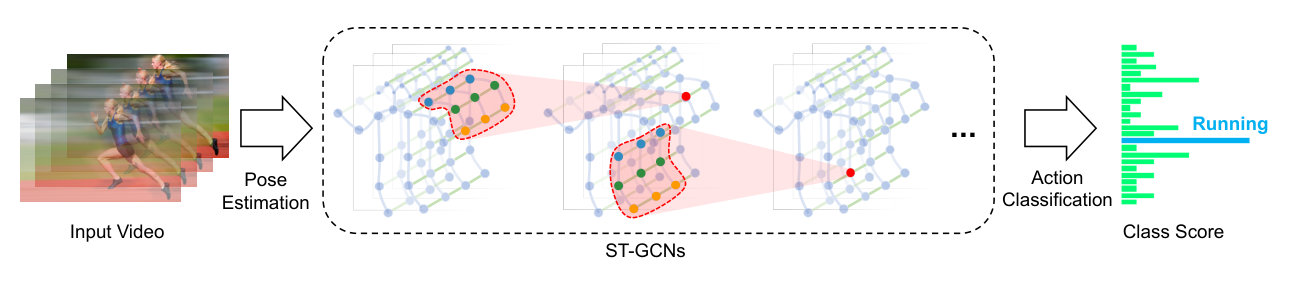
\includegraphics[width=\textwidth]{../ST-GCN-figures/fig1_pipeline_overview.png}
  \caption{Pipeline tổng quát của ST-GCN
  (hình từ bài báo gốc~\cite{yan2018stgcn}): ước lượng tư thế từ video
  đầu vào, xây dựng đồ thị không-thời gian, áp dụng nhiều lớp ST-GCN
  và phân loại bằng Softmax.}
  \label{fig:pipeline}
\end{figure*}

\section{Kiến Trúc ST-GCN}
\label{sec:stgcn}

\subsection{Đồ Thị Không-Thời Gian}
\label{sec:graph}

ST-GCN~\cite{yan2018stgcn} biểu diễn một chuỗi khung xương $N$ khớp
trong $T$ frame dưới dạng đồ thị không định hướng
$\mathcal{G} = (\mathcal{V}, \mathcal{E})$. Tập node
$\mathcal{V} = \{v_{ti} \mid t = 1,\ldots,T;\; i = 1,\ldots,N\}$ gồm
$T \times N$ node, mỗi node ứng với khớp $i$ tại frame $t$. Tập cạnh
$\mathcal{E}$ chia thành hai loại (Hình~\ref{fig:stgcn_graph}):

\begin{itemize}
  \item \textbf{Cạnh không gian} $\mathcal{E}_S$: nối các khớp có kết
    nối giải phẫu trong cùng một frame, phản ánh cấu trúc xương người.
    Chúng ta có $\{v_{ti}v_{tj} \mid (i,j) \in H\}$, trong đó $H$ là
    tập cạnh xương.
  \item \textbf{Cạnh thời gian} $\mathcal{E}_F$: nối cùng một khớp
    giữa hai frame liên tiếp, mã hóa quỹ đạo chuyển động.
    $\{v_{ti}v_{(t+1)i}\}$ cho mọi $t$ và $i$.
\end{itemize}

Đồ thị khung xương 18 node của chúng tôi bao gồm 19 cạnh không gian
giải phẫu (theo cấu trúc COCO-17) cộng thêm 4 cạnh nối node trung tâm
ảo với hai vai và hai hông.

\begin{figure}[!h]
  \centering
  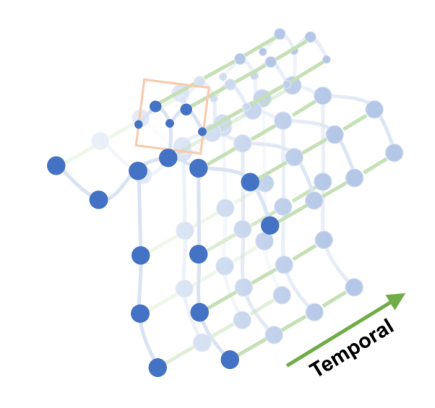
\includegraphics[width=0.85\columnwidth]{../ST-GCN-figures/fig2_spatial_temporal_graph.png}
  \caption{Đồ thị không-thời gian của chuỗi khung xương trong ST-GCN
  (hình từ bài báo gốc~\cite{yan2018stgcn}).
  \textbf{Chấm xanh đậm}: node khớp;
  \textbf{cạnh xanh ngang}: kết nối giải phẫu trong cùng frame ($\mathcal{E}_S$);
  \textbf{cạnh xanh lá chéo}: liên kết thời gian giữa các frame liên tiếp ($\mathcal{E}_F$);
  \textbf{hình chữ nhật cam}: vùng tiếp nhận của một bộ lọc ($D{=}1$).
  Chiều thời gian tăng theo hướng mũi tên.}
  \label{fig:stgcn_graph}
\end{figure}

\subsection{Tích Chập Đồ Thị Không Gian}
\label{sec:gcn}

Trong không gian ảnh 2D chuẩn, tích chập được định nghĩa qua một hàm
lấy mẫu và một hàm trọng số:
\begin{equation}
  f_{\text{out}}(\mathbf{x}) =
    \sum_{h=1}^{K}\sum_{w=1}^{K}
    f_{\text{in}}\bigl(\mathbf{p}(\mathbf{x},h,w)\bigr) \cdot
    \mathbf{w}(h,w),
\label{eq:conv2d}
\end{equation}
trong đó $\mathbf{p}$ liệt kê các điểm lân cận và $\mathbf{w}$ là hàm
trọng số. ST-GCN mở rộng công thức này lên đồ thị bằng cách định nghĩa
lại hàm lấy mẫu trên tập lân cận $B(v_{ti})$ của node $v_{ti}$:
\begin{equation}
  f_{\text{out}}(v_{ti}) =
    \sum_{v_{tj} \in B(v_{ti})}
    \frac{1}{Z_{ti}(v_{tj})}
    f_{\text{in}}(v_{tj}) \cdot \mathbf{w}\bigl(l_{ti}(v_{tj})\bigr),
\label{eq:gcn}
\end{equation}
trong đó $Z_{ti}(v_{tj}) = |\{v_{tk} \mid l_{ti}(v_{tk}) = l_{ti}(v_{tj})\}|$
là số phần tử trong cùng tập phân vùng (chuẩn hóa theo bậc), và
$l_{ti}: B(v_{ti}) \to \{0,\ldots,K-1\}$ là ánh xạ nhãn phân vùng.

\subsection{Chiến Lược Phân Vùng}
\label{sec:partition}

Ánh xạ nhãn $l_{ti}$ quyết định cách chia tập hàng xóm thành $K$ tập
con (Hình~\ref{fig:partitions}). ST-GCN đề xuất ba chiến lược:

\begin{figure*}[t]
  \centering
  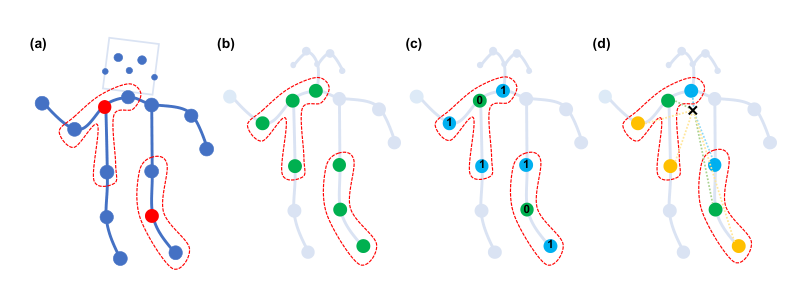
\includegraphics[width=\textwidth]{../ST-GCN-figures/fig3_partition_strategy.png}
  \caption{Ba chiến lược phân vùng của ST-GCN
  (hình từ bài báo gốc~\cite{yan2018stgcn}):
  (a)~ví dụ frame khung xương;
  (b)~Uni-labeling: mọi hàng xóm cùng nhãn (xanh lá);
  (c)~Distance partitioning: node gốc (xanh lá) và hàng xóm (xanh lam);
  (d)~Spatial configuration: hướng tâm (xanh lam) và ly tâm (vàng).}
  \label{fig:partitions}
\end{figure*}

\subsubsection{Uni-labeling ($K = 1$)}
Toàn bộ tập hàng xóm được gán cùng nhãn:
$l_{ti}(v_{tj}) = 0, \; \forall i,j$.
Đây là chiến lược đơn giản nhất, tương đương với lan truyền đồng nhất
của GCN chuẩn~\cite{kipf2017gcn}, nhưng làm mất thông tin về cấu trúc
cục bộ.

\subsubsection{Distance Partitioning ($K = 2$)}
Phân vùng theo khoảng cách đến node gốc: node gốc ở tập $d=0$, hàng
xóm ở tập $d=1$:
$l_{ti}(v_{tj}) = d(v_{tj}, v_{ti})$.
Chiến lược này cho phép mô hình học khác biệt giữa node trung tâm và
các khớp lân cận.

\subsubsection{Spatial Configuration Partitioning ($K = 3$)}
Node hàng xóm được phân vùng dựa trên khoảng cách của nó đến tâm trọng
lực khung xương so với khoảng cách của node gốc:
\begin{equation}
  l_{ti}(v_{tj}) = \begin{cases}
    0 & \text{nếu } r_j = r_i \quad \text{(self-loop / đồng khoảng cách)}\\
    1 & \text{nếu } r_j < r_i \quad \text{(hướng tâm)}\\
    2 & \text{nếu } r_j > r_i \quad \text{(ly tâm)}
  \end{cases}
\label{eq:spatial_config}
\end{equation}
trong đó $r_i$ là khoảng cách trung bình từ tâm trọng lực đến khớp $i$
tính trên toàn bộ tập huấn luyện. Chiến lược này dựa trên quan sát rằng
chuyển động cơ thể có thể được phân tích thành hai thành phần: \textit{hướng
tâm} (chuyển động hướng vào thân người) và \textit{ly tâm} (chuyển động
ra xa thân người), tương ứng với các lớp cơ khác nhau trong sinh lý học
vận động. Đây là chiến lược được sử dụng trong triển khai của chúng tôi.

\subsection{Tích Chập Thời Gian}
\label{sec:tcn}

Sau khi tích chập đồ thị tổng hợp thông tin không gian, một tích chập
thời gian (TCN) với kernel $\Gamma \times 1$ được áp dụng trên chiều
thời gian của mỗi node. Điều này mở rộng khái niệm lân cận lên cả chiều
thời gian:
\begin{equation}
  B(v_{ti}) = \bigl\{v_{qj} \mid d(v_{qj}, v_{ti}) \leq 1,\;
              |q - t| \leq \lfloor\Gamma/2\rfloor\bigr\}.
\end{equation}
Với $\Gamma = 9$ (kernel 9 frame), mỗi node có thể nhìn thấy $\pm 4$
frame xung quanh, cho phép nắm bắt động học cục bộ trong cửa sổ thời
gian $\approx 0.28$ giây (tương ứng 32 fps).

\subsection{Trọng Số Tầm Quan Trọng Cạnh Có Thể Học}
\label{sec:edge_weight}

Một cải tiến quan trọng của ST-GCN so với GCN chuẩn là việc thêm một
ma trận mặt nạ có thể học $\mathbf{M}$ vào mỗi lớp tích chập đồ thị:
\begin{equation}
  \mathbf{f}_{\text{out}} =
    \mathbf{\Lambda}^{-\frac{1}{2}}
    (\mathbf{A} + \mathbf{I})
    \mathbf{\Lambda}^{-\frac{1}{2}}
    \mathbf{f}_{\text{in}} \mathbf{W},
\end{equation}
và đối với phân vùng nhiều tập con:
\begin{equation}
  \mathbf{f}_{\text{out}} =
    \sum_k \mathbf{\Lambda}_k^{-\frac{1}{2}}
    (\mathbf{A}_k \odot \mathbf{M}_k)
    \mathbf{\Lambda}_k^{-\frac{1}{2}}
    \mathbf{f}_{\text{in}} \mathbf{W}_k,
\end{equation}
trong đó $\odot$ là tích Hadamard và $\mathbf{M}_k$ được khởi tạo là
ma trận đơn vị. Ma trận mặt nạ cho phép mô hình tự điều chỉnh tầm quan
trọng của từng cạnh đồ thị theo từng lớp và từng kênh đặc trưng, thay
vì cố định theo cấu trúc giải phẫu. Điều này đặc biệt hữu ích cho Gym99:
trong một số hành động, các khớp chi dưới có thể ít liên quan hơn chi
trên.

\subsection{Kiến Trúc Mạng}
\label{sec:arch}

Hình~\ref{fig:pipeline} minh họa pipeline tổng thể. Kiến trúc cụ thể
trong triển khai của chúng tôi xếp chồng \textbf{9 block ST-GCN}, theo
cấu hình ban đầu của~\cite{yan2018stgcn}. Mỗi block gồm: lớp tích chập
đồ thị (GCN) với phân vùng cấu hình không gian ($K=3$), tiếp theo là
lớp tích chập thời gian (TCN) kernel $9 \times 1$, batch normalization,
và kết nối tắt (residual). Bảng~\ref{tab:arch} tóm tắt cấu hình.

\begin{table}[!t]
\caption{Cấu Hình Các Block ST-GCN}
\label{tab:arch}
\centering
\begin{tabular}{ccccc}
\toprule
Block & Kênh vào & Kênh ra & Stride & Residual \\
\midrule
1 & 2    & 64  & 1 & Không \\
2 & 64   & 64  & 1 & Có    \\
3 & 64   & 64  & 1 & Có    \\
4 & 64   & 128 & 2 & Có    \\
5 & 128  & 128 & 1 & Có    \\
6 & 128  & 128 & 1 & Có    \\
7 & 128  & 256 & 2 & Có    \\
8 & 256  & 256 & 1 & Có    \\
9 & 256  & 256 & 1 & Có    \\
\bottomrule
\end{tabular}
\end{table}

Sau 9 block, \textit{global average pooling} (GAP) rút gọn chiều thời
gian về 1, và một lớp tích chập $1 \times 1$ chiếu vector đặc trưng
256 chiều thành 99 điểm số lớp. Batch normalization đầu vào được áp
dụng trên chiều $C \times V = 2 \times 18 = 36$ để chuẩn hóa tọa độ
đầu vào trước khi truyền vào block đầu tiên.

\subsection{Kiến Trúc Hai Luồng}
\label{sec:twostream}

Luồng joint nhận tensor $\mathbf{X}^{(j)} \in \mathbb{R}^{N \times 2 \times 64 \times 18}$
là tọa độ $(x,y)$ của các khớp. Luồng bone nhận tensor
$\mathbf{X}^{(b)} \in \mathbb{R}^{N \times 2 \times 64 \times 18}$ là
véc-tơ xương: với mỗi cạnh $(u, v)$ trong đồ thị,
$\mathbf{x}^{(b)}_v = \mathbf{x}^{(j)}_v - \mathbf{x}^{(j)}_u$.
Hai mô hình ST-GCN được huấn luyện độc lập với cùng kiến trúc và siêu
tham số. Tại thời điểm suy luận, điểm logit được tổng hợp bằng phép
cộng có trọng số bằng nhau:
\begin{equation}
  \mathbf{s}_{\text{final}} =
    \mathbf{s}^{(j)} + \mathbf{s}^{(b)}.
\end{equation}

Luồng joint nhạy cảm hơn với vị trí tuyệt đối và sự dịch chuyển toàn
cục của khung xương. Luồng bone bổ sung thông tin về tư thế tương đối
(góc khớp và độ dài chi), bất biến hơn với vị trí tuyệt đối. Sự kết hợp
hai nguồn thông tin bổ trợ nhau giúp tăng độ chính xác phân loại,
đặc biệt trong nhận dạng hành động hạt nhỏ nơi sự khác biệt chủ yếu nằm
ở tư thế tương đối chứ không phải vị trí trong không gian.

% ─────────────────────────────────────────────────────────────────────────────
\section{Thực Nghiệm}
\label{sec:exp}

\subsection{Thiết Lập Huấn Luyện}

Mô hình được huấn luyện trên Google Colab và Kaggle với GPU NVIDIA T4.
Optimizer: Adam ($lr = 10^{-3}$, weight decay $= 10^{-4}$); learning
rate scheduler: Linear Warmup 10 epoch tiếp theo Cosine Annealing;
batch size: 64; số epoch: 90; hàm mất mát: Focal Loss
($\gamma = 2,0$, $\alpha$ theo căn bậc hai nghịch đảo tần suất lớp).
Chuẩn hóa bounding-box theo từng mẫu được áp dụng trước khi đưa vào mô
hình.

% TODO: điền kết quả thực nghiệm sau khi hoàn thành huấn luyện đầy đủ

% ─────────────────────────────────────────────────────────────────────────────
\section{Kết Luận}
\label{sec:conclusion}

Chúng tôi đã trình bày ứng dụng ST-GCN hai luồng cho bài toán nhận dạng
hành động thể dục dụng cụ hạt nhỏ trên Gym99 -- một tập dữ liệu quy mô
lớn, nhiều lớp, và mất cân bằng nghiêm trọng. Sự lựa chọn biểu diễn
khung xương 18 node (COCO-17 + trung tâm ảo), chiến lược phân vùng cấu
hình không gian, và hàm mất mát Focal Loss tạo thành một hệ thống tích
hợp chặt chẽ cho bài toán này. Các hướng nghiên cứu tiếp theo bao gồm:
(i)~tích hợp luồng motion (sai phân tọa độ theo thời gian) như trong
các công trình hậu ST-GCN; (ii)~áp dụng ma trận kề có thể học thích
nghi (AGCN) để nắm bắt phụ thuộc ngữ nghĩa vượt ra ngoài cấu trúc
giải phẫu; (iii)~khai thác cấu trúc phân cấp của FineGym (event $\to$
element $\to$ action) thông qua học có giám sát đa nhiệm vụ.

% ─────────────────────────────────────────────────────────────────────────────
\begin{thebibliography}{00}

\bibitem{yan2018stgcn}
S. Yan, Y. Xiong, and D. Lin,
``Spatial Temporal Graph Convolutional Networks for Skeleton-Based
Action Recognition,''
in \textit{Proc. AAAI Conf. Artif. Intell.}, 2018.

\bibitem{shi2019agcn}
L. Shi, Y. Zhang, J. Cheng, and H. Lu,
``Two-Stream Adaptive Graph Convolutional Networks for Skeleton-Based
Action Recognition,''
in \textit{Proc. IEEE CVPR}, 2019.

\bibitem{liu2020msg3d}
Z. Liu, H. Zhang, Z. Chen, Z. Wang, and W. Ouyang,
``Disentangling and Unifying Graph Convolutions for Skeleton-Based
Action Recognition,''
in \textit{Proc. IEEE CVPR}, 2020.

\bibitem{chen2021ctr}
Y. Chen, Z. Zhang, C. Yuan, B. Li, Y. Deng, and W. Hu,
``Channel-wise Topology Refinement Graph Convolution for Skeleton-Based
Action Recognition,''
in \textit{Proc. IEEE ICCV}, 2021.

\bibitem{kipf2017gcn}
T. N. Kipf and M. Welling,
``Semi-Supervised Classification with Graph Convolutional Networks,''
in \textit{Proc. ICLR}, 2017.

\bibitem{bruna2014spectral}
J. Bruna, W. Zaremba, A. Szlam, and Y. LeCun,
``Spectral Networks and Locally Connected Networks on Graphs,''
in \textit{Proc. ICLR}, 2014.

\bibitem{niepert2016learning}
M. Niepert, M. Ahmed, and K. Kutzkov,
``Learning Convolutional Neural Networks for Graphs,''
in \textit{Proc. ICML}, 2016.

\bibitem{shahroudy2016ntu}
A. Shahroudy, J. Liu, T.-T. Ng, and G. Wang,
``NTU RGB+D: A Large Scale Dataset for 3D Human Activity Analysis,''
in \textit{Proc. IEEE CVPR}, 2016.

\bibitem{liu2016spatio}
J. Liu, A. Shahroudy, D. Xu, and G. Wang,
``Spatio-Temporal LSTM with Trust Gates for 3D Human Action Recognition,''
in \textit{Proc. ECCV}, 2016.

\bibitem{kim2017interpretable}
T. S. Kim and A. Reiter,
``Interpretable 3D Human Action Analysis with Temporal Convolutional
Networks,''
in \textit{Proc. IEEE CVPR Workshops}, 2017.

\bibitem{hussein2013covariance}
M. E. Hussein, M. Torki, M. A. Gowayyed, and M. El-Saban,
``Human Action Recognition Using a Temporal Hierarchy of Covariance
Descriptors on 3D Joint Locations,''
in \textit{Proc. IJCAI}, 2013.

\bibitem{wang2012mining}
J. Wang, Z. Liu, Y. Wu, and J. Yuan,
``Mining Actionlet Ensemble for Action Recognition with Depth Cameras,''
in \textit{Proc. IEEE CVPR}, 2012.

\bibitem{vemulapalli2014human}
R. Vemulapalli, F. Arrate, and R. Chellappa,
``Human Action Recognition by Representing 3D Skeletons as Points in a
Lie Group,''
in \textit{Proc. IEEE CVPR}, 2014.

\bibitem{shao2020finegym}
D. Shao, Y. Zhao, B. Dai, and D. Lin,
``FineGym: A Hierarchical Video Dataset for Fine-grained Action
Understanding,''
in \textit{Proc. IEEE CVPR}, 2020.

\bibitem{zhou2023learning}
K. Zhou, Y. Liu, Y. Qiao, and T. Xiang,
``Learning Discriminative Features for Fine-grained Skeleton-Based
Action Recognition,''
\textit{Pattern Recognition}, 2023.

\end{thebibliography}

\end{document}
